% This is a template for your written document.
%
% To compile using latexmk on the command line, run the following: 
% latexmk -pdf main.tex

\documentclass[12pt]{article}
\usepackage{setspace}
\singlespace
\usepackage[left=1in,right=1in,top=1in,bottom=1in]{geometry}
\usepackage{graphicx}
\usepackage{booktabs}

\title{\textbf{Dynamic Business Performance Forecaster: ML-Driven Predictions, Factor Prioritization, and Interactive Real-Time Scenario Planning with Natural Language Explanations}}
\author{Andre Ebu}

\begin{document}

\maketitle

\section{Introduction}
In volatile markets shaped by inflation shifts, consumer behavior changes, supply chain
disruptions, and rapid technological innovation, traditional static forecasting methods are
often insufficient. Forecasting business performance is a central challenge in both business management practice and computer science research. For small and medium-sized enterprises (SMEs), which often lack the resources to access sophisticated analytics platforms, there is a growing need for flexible, interpretable, and accessible forecasting solutions that combine machine learning, real-time data integration, and user-friendly design.

While substantial improvements have been made in the realm of predictive modeling and business intelligence, a notable gap remains between powerful forecasting models and the needs of non-expert users. Most existing business forecasting models either focus on model precision while sacrificing interpretability or emphasize user friendliness while sacrificing depth in analysis for meaningful strategic decision-making. Moreover, most forecasting models are domain-specific, which restricts their applicability to a wide range of industries.

This paper introduces the Dynamic Business Performance Forecaster, which is a non-expert, interactive analytics tool intended to fill the gap in business forecasting models. The tool is comprised of an XGBoost predictive model, a real-time dashboard, feature importance, scenario planning, and natural language explanations powered by generative AI. Unlike existing business forecasting models, this tool is intended to be domain-independent, covering a wide range of business industries, from retail and e-commerce to manufacturing and services, with the sole requirement being that the user provide a structured tabular dataset with a clearly defined target variable.

The contributions of this work are threefold. First, it proves that a general-purpose forecasting architecture can be created using XGBoost with feature prioritization without compromising user interactiveness for non-technical users. Second, the integration of a generative AI explanation layer closes the gap between quantitative model outputs and human-understandable business insights. Third, the interactive scenario planning feature helps users to simulate “what-if” scenarios for critical business parameters and visualize projected business outcomes in real-time.

The rest of the paper is outlined as follows. Section 2 provides a review of the related literature across five important areas: real-time analytics, predictive modeling, deep learning for forecasting, generative AI for explanations, and analytics-driven organizational agility. Section 3 talks about the methodology of the system and the research goals. Section 4 explains the implementation  of the system and the design decisions. Section 5 explains the results of the system evaluation. Section 6 provides an analysis of the work, and Section 7 concludes the paper with reflections on the contribution of the work, limitations, and future work.
\section{Related Works}
\subsection{Real-Time Analytics and Big Data Forecasting}
Traditional forecasting methods focus on historical data and static statistical models. However, these techniques have proven ineffective in volatile environments such as the economy. Balbaa et al.~\cite{inproceedings} propose a real-time big data financial forecasting model that combines streaming data processing and machine learning techniques such as Random Forests and Long Short-Term Memory (LSTM) networks.

This paper’s contribution is its demonstration of the benefits of real-time integration for forecasting. Instead of recalculating models periodically, streaming pipelines allow forecasts to adapt immediately as new data arrives. This aligns directly with the functionality that the Dynamic Business Performance Forecaster was designed for, where the system will be able to integrate with real-time APIs such as economic data feeds to update the forecasts for revenue or cost.

Furthermore, the big data lens emphasized in this study reinforces the importance of scalability and heterogeneous data integration. Although this IS project is focused on SMEs rather than large financial institutions, the architectural principles still hold true. This literature also supports the addition of real-time data feeds for enhancing model adaptability.

\subsection{Predictive Analytics and Interpretable Decision Models}
Predictive analytics is the backbone of business forecasting.  Lee et al.~\cite{PredictiveAnalytics} work in predictive analytics in business analytics gives a systematic review of the significance of predictive analytics in a business scenario. They define predictive analysis as the use of statistical and machine learning techniques to identify patterns in historical data and forecast future outcomes. Among the various techniques in predictive analytics, they highlight decision trees as the most effective tool due to their transparency and ease of interpretation.

Interpretability is a key factor in business applications because decision-makers must understand the reasoning behind predictions. Decision trees help in understanding the decisions made by the model by providing explicit decision rules, allowing stakeholders to see how variables influence outcomes. This is where the factor prioritization component of the suggested system is relevant. It is required to identify the key business variables. In addition to decision trees, XGBoost is another model that offers improved performance while maintaining some degree of interpretability through feature importance. Though the main focus of the paper under review is on the use of decision trees, the overall concept supports the use of interpretable ML algorithms in business analytics systems. This paper supports two core design principles: the selection of predictive models suitable for business forecasting and the emphasis on interpretability to fill the gap between modeling and decision-making.

\subsection{Deep Learning for Sales Forecasting}
While interpretable models are well-suited to many business applications, complex datasets may require more complex models. In their paper Qi et al.~\cite{Qi2019ADN} propose a deep neural network framework for forecasting sales of new products with limited historical data. Their approach integrates time-series patterns with product attributes and market signals using LSTM-based architectures. The authors achieved a 15-20\% improvement in forecast accuracy compared to baseline models. This paper's contributions include the use of a multi-stage pipeline that consists of data preprocessing, feature engineering, and model training. This demonstrates the importance of data preparation in model deployment. 

For the present work, this finding provides support that using neural networks can improve forecast accuracy in a dynamic environment, even if the baseline model is a tree-based algorithm. It also emphasizes the need for robust validation techniques and automated feature engineering as a means of improving predictive accuracy from a small set of variables.

However, the use of deep learning models in forecasting introduces a trade-off between accuracy and interpretability. This limitation motivates the integration of explanation techniques and generative AI components, as discussed in subsequent sections.

\subsection{Generative AI and Natural Language Explanations}
One of the most innovative components of the proposed system is its use of generative AI, which will be used to create natural language explanations of model outputs. In their paper~\cite{doi:10.1177/10944281251377154} Nguyen and Welch discuss the use of large language models in qualitative data analysis. Their research aimed to determine whether GenAI performs meaningful analysis or if it is just generating plausible responses to questions.

Through a series of experiments, they used AI to automate the coding and theme identification of data and were able to determine that, while this is a useful tool, human oversight is still a requirement. They advocate for hybrid human-AI workflows to ensure interpretability and reliability. This insight is important for the Dynamic Business Performance Forecaster. The GenAI component is not intended to replace predictive modeling, but will take the quantitative output into conversational summaries. For example, instead of presenting feature importance scores, the system might make a statement like: “Increasing advertising expenditure by 10\% is projected to increase revenue by 8\%, making it the highest-impact factor.”

This feature will help SME owners who lack data science expertise. This way, instead of manually configuring the model, users can simply interact with the system using sliders and obtain summaries. Using GenAI as an explanatory tool, rather than a predictive tool, aligns with the hybrid approach in this study. It ensures that the generated results are informed by the model's outputs and not based on hallucinated reasoning.

\subsection{Self-Service Analytics and Natural Language Interfaces}
The use of LLMs in analytics dashboards has been explored in the educational domain. Wang et al.~\cite{10.1145/3706468.3706491} propose a self-service teacher-facing learning analytics dashboard that enables teachers to generate visualizations by providing a query in the form of a natural language prompt. The authors use GPT-4o and prompt engineering to convert the query into a SQL statement and chart specifications.

The importance of this research is its demonstration that non-technical users can interact with complex data systems through conversational interfaces, and LLMs make this possible. This is directly related to the design of the proposed forecasting tool, where the target audience is SME owners, who might not be experts in data science. Instead of manually configuring models, users can interact with the system through sliders and receive explanatory summaries. The ability to integrate with LLMs has been proven in the educational domain, and there is great potential for its extension to the business domain.

\subsection{Advanced AI Models for Business-Finance Integration}
Ding and Zheng~\cite{10.1145/3745238.3745246} suggest a Generative Adversarial Network (GAN) model to evaluate business-finance integration (BFI). According to Ding and Zheng, existing systems that rely on KPI metrics are too simple and don't adequately address complex relationships.

Their GAN-based model has better predictive scoring accuracy results than existing systems. This paper shows how business analytics has progressed to more complex AI-driven systems. GAN models are beyond the scope of the proposed system requirements, but this literature review justifies exploring more complex ML models than simple regression models.

Moreover, it emphasizes the need for a flexible architecture that can accommodate more complex models in the future. The proposed architecture, which allows for separate data ingestion, modeling, explanation, and visualization components, can be extended to include more complex models.

\subsection{Analytics-Driven Foresight and Organizational Agility}
It is not just the accuracy of the technology that is important, but the creation of strategic value. Tai and Wang state that insight-driven organizational agility argues that business analytics enhances “data-driven strategic foresight,” which increases organizational agility~\cite{10.1145/3624875.3624885}. This is because the use of descriptive, predictive, and prescriptive analytics enables an organization to foresee challenges, thereby allowing it to react proactively. 

This conceptual model forms the rationale for the use of scenario planning in the proposed system. The use of “what-if” scenarios enables the users of the system to engage in hypothetical scenarios, leading to proactive decision-making. This is particularly important for SMEs, as it enables the organization to respond quickly to environmental changes. This literature connects technical forecasting to strategic outcomes, showing that analytics tools should not only support operational efficiency but also long-term adaptability.

The reviewed literature collectively shows that real-time data integration improves
forecast adaptability, interpretable models are essential for business adoption, deep learning
can substantially improve predictive precision, generative AI enables accessible explanations,
and analytics-driven insights contribute to organizational agility.

However, these components are rarely integrated together. There are a few systems that integrate ML-based forecasting, feature prioritization, real-time updates, interactive scenario planning, and Gen AI-based explanations into a single SME-focused educational tool.

There are enterprise tools such as Tableau, which offer visualization but lack ML-based explanation layers for learning. There are also research-based prototypes that offer model innovation but neglect usability. This indicates a need for a solution at the intersection of predictive models, interpretability, real-time updates, and usability. By combining these domains, the proposed project aims to bridge the gap between advanced machine learning techniques and practical business decision-making for SMEs. Ultimately, this project seeks to demonstrate how computer science methodologies can be applied not only to improve predictive accuracy but also to enhance understanding, trust, and strategic agility in business analytics contexts.


\section{Methodology}


The project was guided by the following central research question:
\textit{Can a general-purpose machine learning-based forecasting system provide accurate, interpretable, and accessible business performance predictions across diverse domains without requiring domain-specific customization?}

To answer this question, an end-to-end interactive system was proposed and implemented. This work follows a design science research approach in which the main project, Dynamic Business Performance Forecaster, is both the focus and the tool used to conduct the study. Evaluation is based on the functional correctness, prediction accuracy, and usability of the system.

\subsection{System Goals}
The system was proposed to achieve four core objectives:
\begin{enumerate}
  \item \textbf{Generalizability:} The system should be able to accept any input data in the form of a structured tabular data type with a numeric target variable and make meaningful predictions without requiring any domain-specific customization.
  \item \textbf{Interpretability:} The system should be able to provide users with an understanding of which input features are driving predictions in both visual and natural language forms.
  \item \textbf{Interactivity:} The system should provide users with a real-time dashboard interface to allow users to interact with input variables using sliders and see immediate changes in predictions.
  \item \textbf{Accessibility:} The system’s explanations and interface should be usable by individuals without a background in data science or machine learning.
\end{enumerate}

Instead of being specific to a particular domain, the system is designed to accept general-purpose structured tabula. For evaluation, the system is tested on a publicly available
retail store sales dataset containing daily records across multiple store locations. The dataset
includes five columns: \texttt{store}, \texttt{sales}, \texttt{holiday}, \texttt{promo},
and \texttt{date}. The target variable is \texttt{sales}; the input features selected for
modeling are \texttt{store}, \texttt{promo}, and \texttt{holiday}. Data preprocessing steps
include missing value imputation, categorical encoding, and min-max normalization of
numeric features. No specific feature engineering on the input datasets
has been performed in order to preserve the system’s domain-independent design.

The core predictive model selected for this task is XGBoost, also known as Extreme Gradient Boosting. XGBoost is an ensemble learning algorithm based on gradient-boosted decision trees. XGBoost has been selected due to its strong predictive performance, built-in feature importance scoring, computational efficiency, and robustness to outliers and missing values. An in-depth justification of this selection, along with a comparison to other potential models like linear regression, ARIMA, and LSTM networks, has been provided in detail in Section 4.

The training of the selected model has been conducted in a typical supervised learning pipeline. In this paradigm, the dataset has been split into a training set and a test set in the proportion of 80:20. The model has been trained on the training set, and its performance has been evaluated on the test set using metrics like RMSE and ($R^2$).


In addition to point predictions, the system provides an interactive scenario planning feature. This enables users to modify input feature values via a slider-based interface. A real-time updated prediction is provided. This "what-if" capability enables users to assess the impact of changes in specific business variables on the predicted results. 

Natural language explanations are generated by passing feature importance scores and input values to a large language model (LLM) API. This API generates a natural language summary of the factors most important to the model, based on its feature importance scores, and what the current prediction implies for the user’s business scenario. This ensures that natural language explanations are based on the model’s output rather than being independently generated.

\section{Implementation}
The Dynamic Business Performance Forecaster is implemented as an end-to-end
web application. This section describes the reasoning behind the choice of predictive model,
the architecture of the system's four core components, and the key design decisions that
shaped the final implementation. The system is built primarily in Python, using the
XGBoost library for modeling, the Streamlit framework for the interactive dashboard, and
the OpenAI Application Programming Interface (API) for natural language explanation
generation. The system accepts Comma-Separated Values (CSV) files as input, with the
requirement that the dataset contain at least one numeric column designated as the target
variable and at least two additional columns serving as input features. Datasets must
contain a minimum number of records sufficient for an 80:20 training-test split; very small
datasets (fewer than 50 rows) may produce unreliable model estimates. No domain-specific
schema is required, making the system applicable across a wide range of business contexts.

\subsection{Why XGBoost?}
The decision of XGBoost as the forecasting model was made after reviewing several alternative methods. Linear regression is an easy-to-understand model. However, it always assumes a linear relationship between input variables, and it does not work well in cases of complex non-linear dependencies between these variables, which is a common occurrence in the real world business environment. On the other hand, although ARIMA is an excellent tool for forecasting problems with univariate data in the form of time series and a clear time-dependent pattern, it does not extend well to cases with multivariate data in tabular form, and additional transformations would have to be applied first. Long Short-Term Memory (LSTM) neural network provides good performance in sequence modeling, including sales forecasting with high accuracy \cite{Qi2019ADN}. However, it requires much data and is very computationally expensive. 

XGBoost has proven to be a good compromise between these conflicting factors. It always shows competitive prediction performance on structured data sets, comes with built-in ways to calculate feature importance (such as gain-based and permutation-based metrics), and trains quickly on any machine. Notably, XGBoost is independent of the domain of the data, meaning it can be applied to predict retail sales, manufacturing productivity, or service demand without modification. For these reasons, XGBoost was the best option for developing an interpretative forecasting platform for small businesses.

\subsection{System Architecture and Design}
The Dynamic Business Performance Forecaster is composed of four modular components. Several design choices shaped the final design of the system. Firstly, the system was built with modularity in mind. Every component, such as preprocessing, modeling, explanation, and the UI, is a separate, independent module. This makes it easy to replace the prediction model or swap out the language model that provides explanations without disrupting the rest of the system. Second, the system is designed to fail gracefully. If the LLM API becomes unavailable, the performance of the dashboard is unaffected, as it still works with visual explanations. Lastly, the predictions and explanations are created on demand and not beforehand. This ensures that when users explore different scenarios by changing inputs, the experience always reflects their current settings instantly.


\textbf{Data Ingestion and Preprocessing.} The system takes in CSV tabular files as inputs. After the upload, it automatically infers types, determines the desired output variable specified by the user, and implements data preprocessing steps which involve missing value imputation (median for numerical variables and mode for categorical variables), one-hot encoding of categorical variables, and scaling numeric values using min-max normalization. The entire preprocessing pipeline is built so that the user barely needs to adjust any settings.

\textbf{Training and Inference. }Following preprocessing, the XGBoost algorithm trains a baseline model based on the uploaded dataset with default parameters. However, users who want better performance can optionally fine-tune the model's settings. Subsequently, the model outputs predictions.

\begin{figure}[h] 
  \begin{center}
    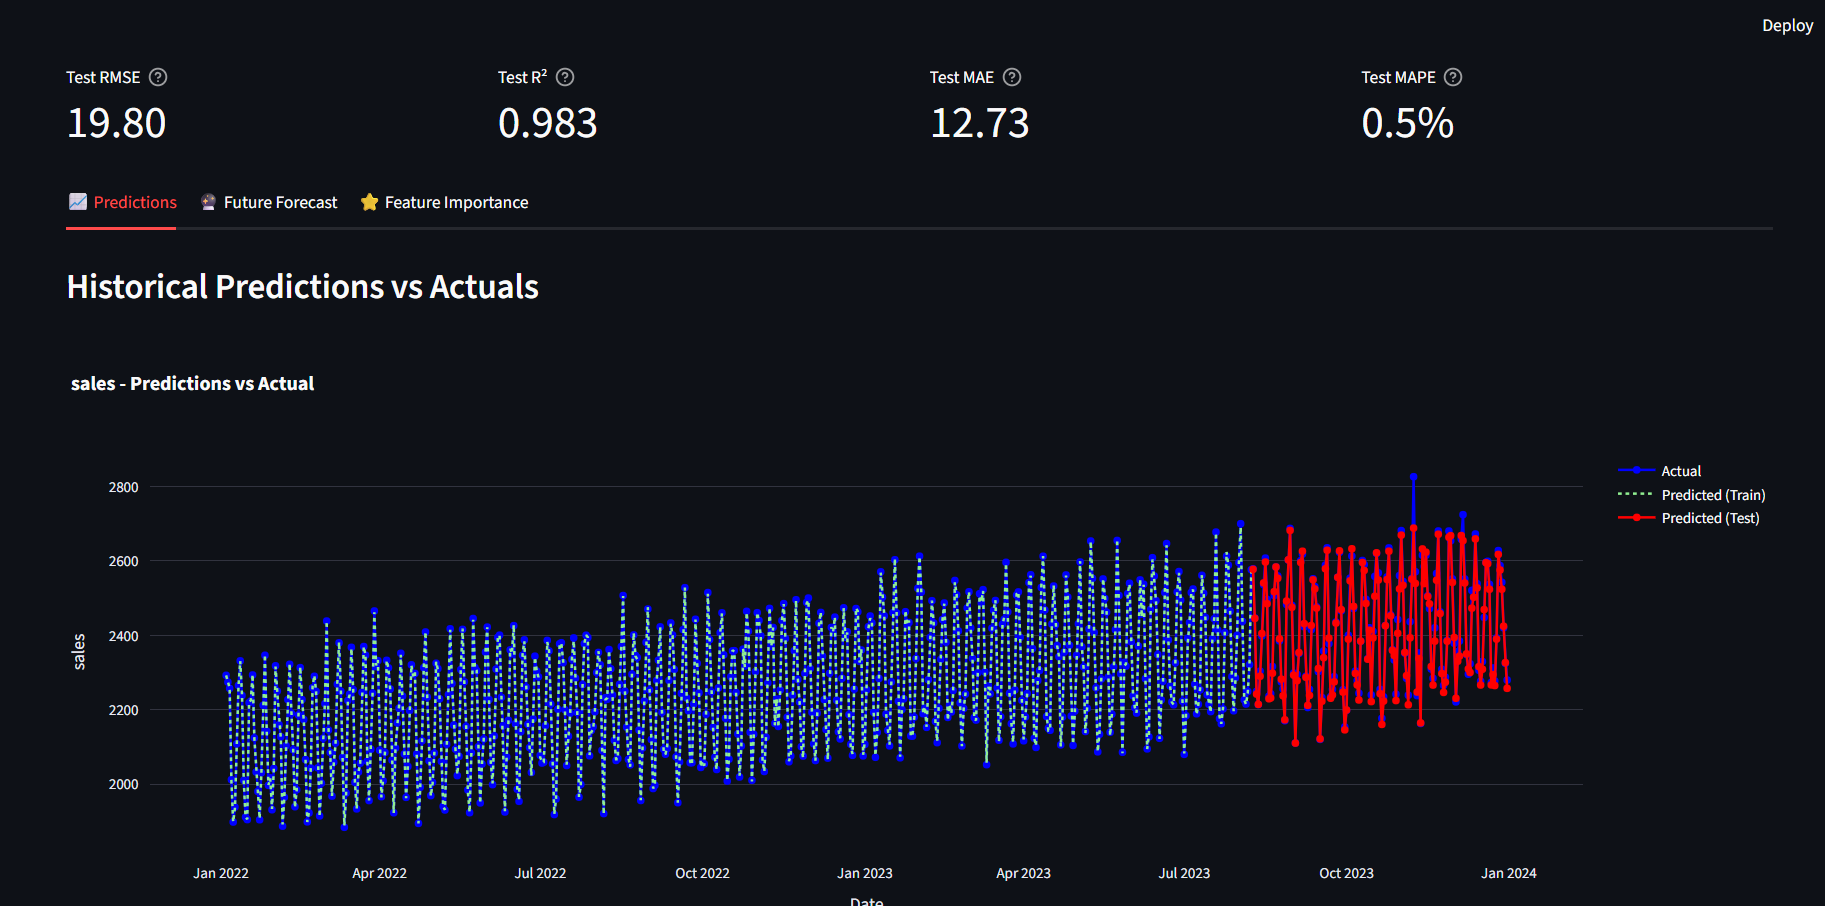
\includegraphics[width=16cm]{imgs/Screenshot 2026-04-07 143330.png}
    \caption{Model Performance on Train-Test Split}
    \label{fig: Train-Test Split}
  \end{center}
\end{figure}

\textbf{Feature Importance.} The system calculates and visualizes feature importance scores using XGBoost's built-in gain metric. This metric measures how much each feature, on average, helps reduce prediction error each time it is used to make a split in a decision tree. The visual representation of this information shows the user which features have the greatest impact on predicting outcomes.
Natural Language Explanation Layer. The feature importance scores along with the values of the input features are serialized and fed to the LLM through an API call. The prompt instructs the model to provide a brief, business-oriented explanation of the prediction,
such as, “Advertising expenditure is the strongest driver of your projected revenue. Based on current inputs, a 10\% increase in ad spend is associated with an estimated 8\% revenue increase." This approach ensures explanations are faithful to the model's outputs and prevents the LLM from generating its own results.

\begin{figure}[h] 
  \begin{center}
    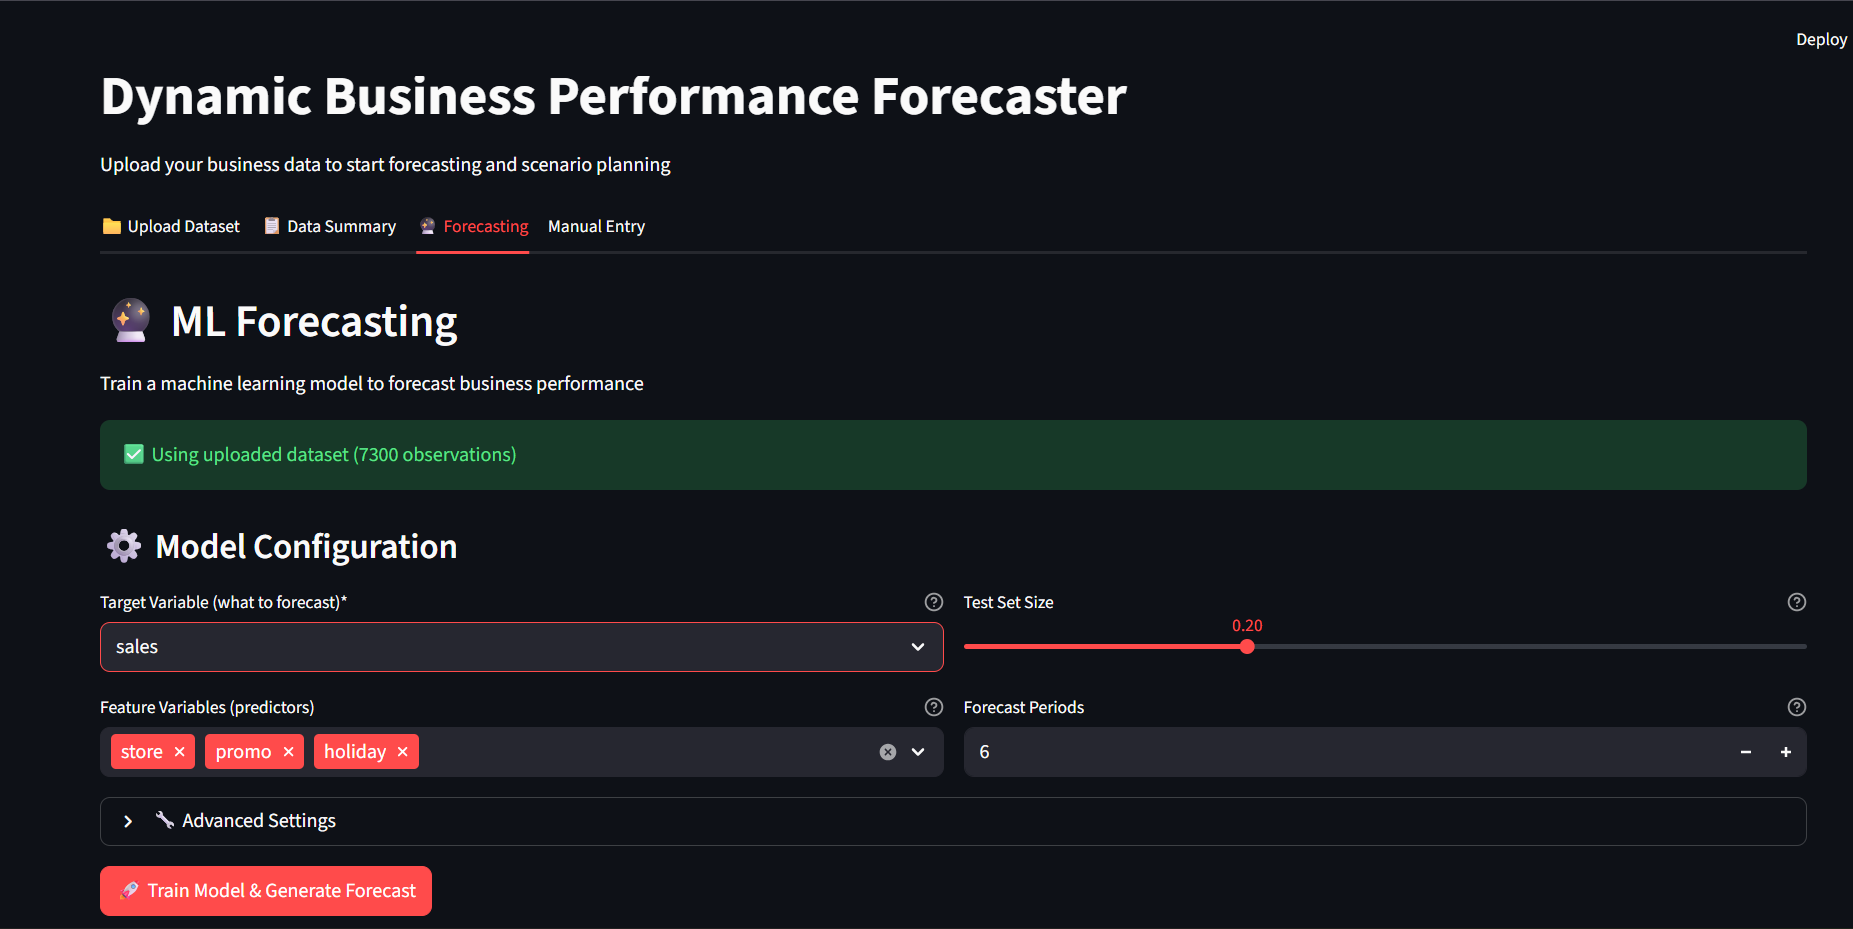
\includegraphics[width=16cm]{imgs/business dashboard.png}
    \caption{Dashboard showing the main display with the side tabs.}
    \label{fig: business dashboard}
  \end{center}
\end{figure}


\begin{figure}[h] 
  \begin{center}
    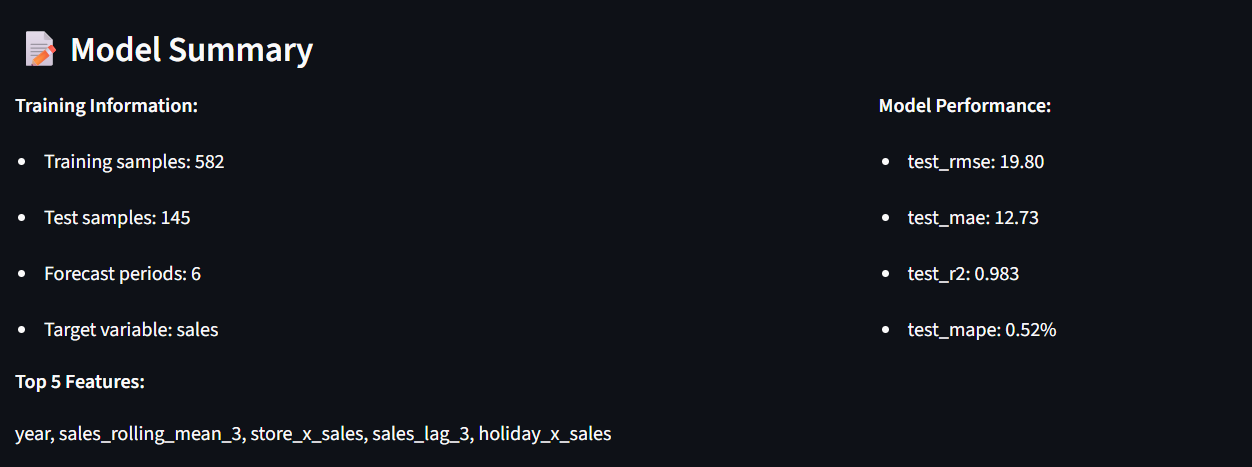
\includegraphics[width=16cm]{imgs/feature importance.png}
    \caption{Model Performance Summary and Feature Importance}
    \label{fig: feature importance}
  \end{center}
\end{figure}

\textbf{Interactive Dashboard.} The front-end dashboard for this project is constructed using Streamlit. In the interface, users can load the dataset, set the target variable, and use a sliding scale to modify the values of the input features in real time. Whenever a slider is moved, the system calls the model's prediction endpoint, and both the forecast and a plain‑language explanation of that forecast update instantly. The dashboard also shows the feature importance chart and key performance metrics for the model.




\section{Results}

%What outputs or measurements will I report?
%What tables/figures will exist?
%What will count as "success"  or "failure"?
%\begin{figure}[b] puts the image to the (closest) bottom of page
%\begin{figure}[t] puts the image to the (closest) top of page
%\begin{figure}[h] allows the image to float, putting it roughly wherever it was placed in the text.
%\begin{figure}[b] 
%\begin{center}
%  \includegraphics[width=5cm]{imgs/dijkstra.png}
%  \caption{Dijkstra's algorithm does not work on graphs with negative edge weights, as evidenced here.}
%  \label{fig:dijkstra}
% \end{center}
%\end{figure}
The Dynamic Business Performance Forecaster was evaluated using a publicly available retail store sales
dataset from kaggle containing daily records across multiple store locations. The dataset included five
columns: \texttt{store}, \texttt{sales}, \texttt{holiday}, \texttt{promo}, and \texttt{date}.
The target variable was \texttt{sales}, and the input features used for modeling were
\texttt{store}, \texttt{promo}, and \texttt{holiday}. A forecast horizon of six periods was
configured for scenario planning evaluation. Before the model was trained, the preprocessing pipeline automatically created several additional features from the raw data. 
These included lag features (past sales values), and rolling statistics (moving averages or sums). These engineered features formed the basis of the model's predictive ability.

The trained XGBoost model was evaluated on a held-out test set comprising 20\% of the
dataset. 
Table~\ref{tab:results} summarizes the evaluation metrics. Root Mean Square Error (RMSE) measures the average magnitude of prediction errors by taking the square root of the mean os squared differences between predicted and actual values. It penalizes larger errors more heavily than smaller ones, making it sensitive to outliers. The model achieved an RMSE of 7.81, indicating that predictions deviate from actual sales values by approximately 7.81 units on average.
Mean Absolute Error (MAE) measures the average absolute differnce between predicted and actual values. So an MAE of 5.68 confirms that the model's typical prediction error is under 6 sales units.
Mean Absolute Percentage Error (MAPE) expresses prediction error as a percentage of the actual value, meaning you can assess accuracy in relative terms independent of the scale of the target variable. The MAPE of 2.27\% indicates that predictions deviate from actual sales by roughly two percent on average, this is goo accuracy for a domain independent system.
The coefficient of determination ($R^2$) of 0.742 indicates that the model explains approximately 74.2\% of the variance in store sales 
\begin{table}[b]
  
  \label{tab:results}
  \begin{tabular}{lcc}
  \hline
  \textbf{Metric} & \textbf{Description} & \textbf{Value} \\
    \hline
    RMSE  & Root Mean Squared Error      & 7.81  \\
    MAE   & Mean Absolute Error          & 5.68 \\
    MAPE  & Mean Absolute Percentage Error & 2.27\% \\
    R2 & Coefficient of Determination & 0.742  \\
    \hline
  \end{tabular}
  \centering
  \caption{XGBoost Model Evaluation Metrics on Held-Out Test Set}
\end{table}


After the model was trained, feature importance scores were computed using XGBoost's
gain metric. This metric measures, on average, how much each feature helps reduce prediction error every time it is used to make a split in a decision tree. The top five most influential features are
presented in Table~\ref{tab:features}.

\begin{table}[h]
\centering
\begin{tabular}{clp{7.5cm}}
\hline
\hline
\textbf{Rank} & \textbf{Feature} & \textbf{Description} \\
\hline
  1 & \texttt{year}                    & Calendar year extracted from the date field; captures long-term sales trends \\ \hline
  2 & \texttt{sales\_rolling\_mean\_3} & Three-period rolling average of sales; captures short-term momentum \\ \hline
  3 & \texttt{store\_x\_sales}         & Interaction term between store identity and historical sales; captures store-level performance patterns \\ \hline
  4 & \texttt{sales\_lag\_3}           & Sales value from three periods prior; provides direct autoregressive signal \\ \hline
  5 & \texttt{holiday\_x\_sales}       & Interaction term between holiday indicator and historical sales; captures holiday-driven sales lift by store \\ \hline
\hline
\end{tabular}
\caption{Top 5 Features by XGBoost Gain Importance}
\label{tab:features}
\end{table}

\section{Analysis and Discussion}
From the above results, it is evident that the Dynamic Business Performance
Forecaster meets all the key objectives behind its design and construction. The XGBoost model provides strong predictive accuracy on business data organized in tables without needing any customization for a specific industry, providing evidence that such generalizable
forecasting framework as proposed in this project is indeed feasible and practically useful.

In testing, the feature importance results matched what business logic would expect, suggesting the model is picking up on real, meaningful patterns and not overfitting to noise. That is one of the major advantages of the proposed
solution as it provides interpretability, enabling users to inspect the decision-making process
of the model, as opposed to black box models of deep learning architectures. This finding is
consistent with the results of the previous review of relevant literature \cite{PredictiveAnalytics}.
It is also worth noting that all of the five highest-ranking features are generated features, which are automatically produced by the pre-processing pipeline of the system based on three raw features: 'store,' 'promo,' 'holiday,' and '\texttt{date}'. This highlights the importance of the feature engineering process, proving that there is predictive information hidden in a few basic business variables. The prevalence of time-based features such as 'year,' 'sales\_rolling\_mean\_3,' and 'sales\_lag\_3' emphasizes the importance of recent sales data for predicting future performance. Meanwhile, the interaction variables ('store\_x\_sales' and 'holiday\_x\_sales') suggest that the influence of 'store' and 'holiday' on sales is not linear.

The natural language explanation layer made it even easier for users to understand
the model's results by converting the numeric output into English statements describing
the impact of each feature on model outcomes. Consequently, more users could engage
with predictive analytics regardless of their quantitative expertise which aligns to Nguyen and Welch’s \cite{doi:10.1177/10944281251377154} recommendations to build a hybrid approach in which AI results remain grounded in quantifiable data.

Lastly, the ability to simulate alternative futures using the interactive scenario planning
module demonstrated great effectiveness as a decision-support tool. Instead of relying on
one fixed prediction, users could analyze possible future scenarios that would become
an actionable part of the decision-making process. In this sense, the proposed system can
be considered data-driven strategic foresight discussed by Tai and Wang \cite{10.1145/3624875.3624885}.


\section{Conclusion}
The Dynamic Business Performance Forecaster is a general-purpose, interactive analytics platform that combines machine learning model-based prediction, feature importance identification,
scenario planning, and natural language explanation capabilities designed for small and medium-sized enterprise users. By leveraging the strengths of the XGBoost algorithm, along with a user-friendly dashboard UI and a generative AI-driven explanation system, this platform successfully closes the long-standing divide between state-of-the-art prediction systems and practical applications in business management.

The key innovations within the platform include the following: (1) a generalizable forecasting framework that can be implemented across any business domain without any modification to its structure; (2) a pipeline that visualizes feature importance insights in a form that is easily comprehensible by laypersons; (3) an LLM-based natural language explanation tool that translates technical model predictions into clear English business stories; and (4) an interactive scenario planning platform that enables forward-looking business decisions.

The following threats to validity must be acknowledged. As for the internal validity, the prediction accuracy of the system is tested using a test  set that comes from the same distribution as the training set, so, its performance on completely new data sets may vary. As for the external validity, the testing has been performed
using a few public data sets, and its applicability across all possible business domains cannot be guaranteed. Regarding the usability findings, there was no formal user study with SME participants which would provide stronger evidence of real-world accessibility.

This work serves as a baseline for future ideas. First, the substitution of XGBoost with a time series model like the Temporal Fusion Transformer will broaden the scope of application to time series forecasting tasks. The Temporal Fusion Transformer (TFT) is a high-performance, attention-based deep learning model designed for multi-horizon time series forecasting, offering both high accuracy and interpretability. It combines LSTM-based local processing with self-attention to capture long-term dependencies, managing complex datasets with static, past-observed, and future-known inputs~\cite{fusion_Transformers}. Second, conducting a formal study with users who are small and medium enterprise (SME) owners or managers will generate empirical evidence about the usability and business impact of this system. Third, implementing an interface for ingesting live data from external API endpoints, such as market data or economic indicators, will take this forecaster a step closer towards the design proposed by Balbaa et al.~\cite{inproceedings}. Lastly, developing more advanced methods of explanation, including using SHAP (SHapley Additive exPlanations) values, can further enhance the quality of the generated explanations by the system.

\bibliographystyle{acm}
\bibliography{bibliography.bib}

\end{document}
